\newpage
\section{Diophantus---Fermat---Wiles}

Long before the invention of algebra, the Greek mathematician
constructed and solved riddles with whole numbers, several of which
are described in today's sketch.  Fermat had algebra at his disposal
and so was so taken with the number-riddles of Diophantus that he
recorded (and solved) many of them as equations where the solution
numbers should all be whole numbers (integers).  These have come to be
known as Diophantine equations.

\begin{prob}
One problem was to give all solutions to the Diophantine equation
\[
X^2 + Y^2 = Z^2
\]
remembering that $X$, $Y$, and $Z$ all have to be integers.
Diophantus would have asked ``Make a list of all the square numbers
that are the sum of two square numbers.''  Explain why this is the
same problem as solving 
\[
x^2 + y^2 = 1
\]
where $x$ and $y$ are rational numbers.
\end{prob}


\begin{prob}
In the plane below, draw the real-number solution set of $(x,y)$ so
that $x^2 + y^2 = 1$.
\begin{enumerate}
\item Find one rational-number solution $C = (x,y)$ to the equation such that neither $x$ nor $y$ is $0$.  Plot your solution $C$ in the plane below.
\item Draw the line through your solution and the solution $A = (0,1)$.  Mark the point $B$ at which your line crosses the $x$-axis.
\item Find the $x$-coordinate of $B$.  Is it a rational number?  Why or why not?
\end{enumerate}
\[
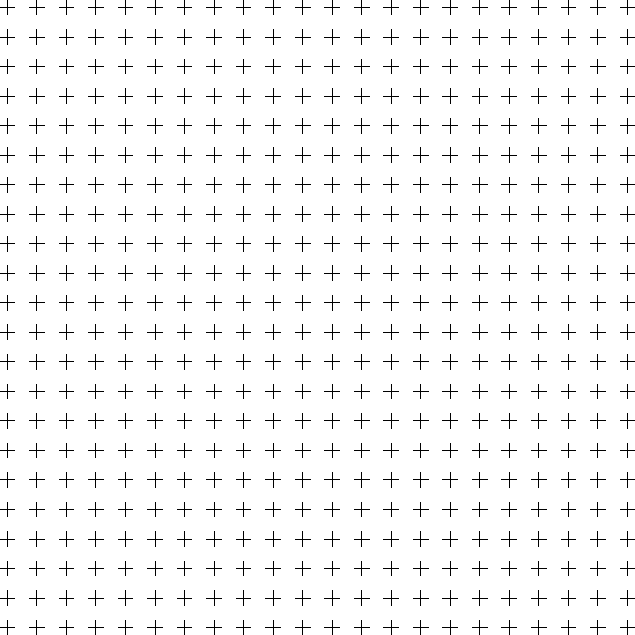
\includegraphics{../graphics/complexPlane.pdf}
\]
\end{prob}

\begin{prob}
Now on the grid below,
\begin{enumerate}
\item Draw the real-number solution set $x^2+y^2 = 1$, and mark the point $A' = (0,1)$.
\item Mark any point $B' = (r,0)$ inside the circle on the $x$-axis such that $r$ is a rational number.
\item Draw the line through $A'$ and $B'$.
\item Find the coordinates of the other point $C'$ at which your line cuts the solution set $x^2+y^2 =1$.  Are they rational numbers?  Why or why not?
\end{enumerate}
\[
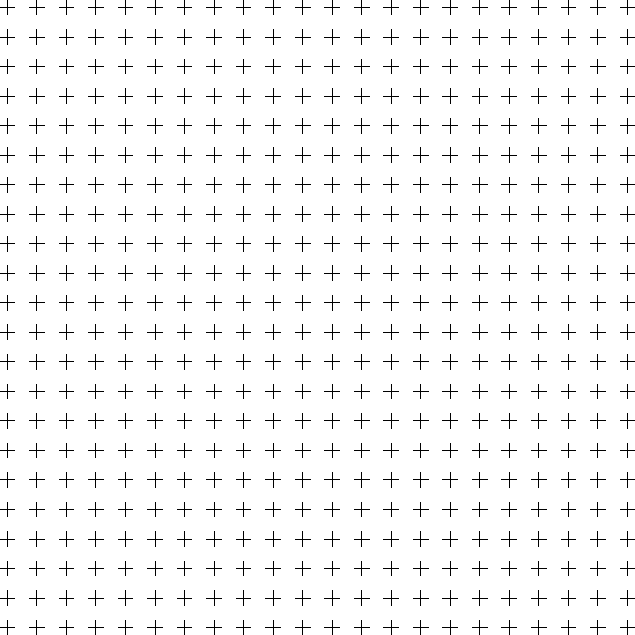
\includegraphics{../graphics/complexPlane.pdf}
\]
\end{prob}

\begin{prob}
Turn your solution $C'$ in the problem above into an integer solution
to the equation $X^2 + Y^2 = Z^2$.
\end{prob}

